\documentclass{cornouaille}
\usetikzlibrary{matrix,arrows,decorations.pathmorphing}
% l' unité
\newcommand{\myunit}{1 cm}
\tikzset{
    node style sp/.style={draw,circle,minimum size=\myunit},
    node style ge/.style={circle,minimum size=\myunit},
    arrow style mul/.style={draw,sloped,midway,fill=white},
    arrow style plus/.style={midway,sloped,fill=white},
}
\newcommand{\touchecalc}[1]{\fbox{#1}}
\impression
\begin{document}
\fexo{TS-Spé-C2}{Calcul matriciel}{Année 2018-2019}

\tableofcontents

\section{Définitions et vocabulaire}

%Dans tout ce chapitre, sauf indication contraire, $m$, $n$ , $p$, $i$ et $j$ désignent des entiers naturels non nuls.

 \begin{definition}[Matrice]
Une \textbf{matrice} de \textbf{taille} $m\times n$ est un tableau de nombres formé de $m$ lignes et $n$ colonnes qui s’écrit sous la forme :
\begin{center}
	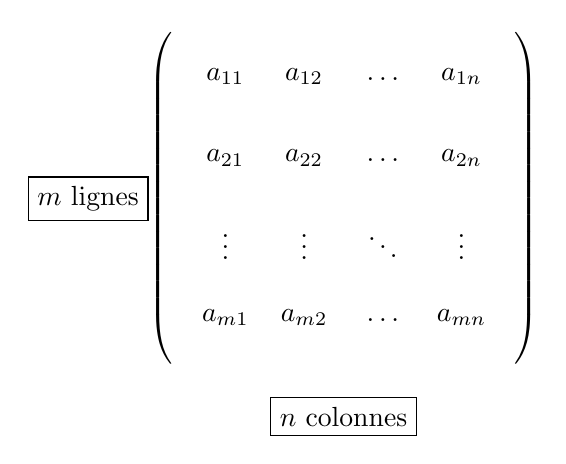
\begin{tikzpicture}[>=latex]
% les matrices
\matrix (A) [matrix of math nodes,%
             nodes = {node style ge},%
             left delimiter  = (,%
             right delimiter = )] at (0,0)
{%
  a_{11} & a_{12} & \ldots & a_{1n}  \\
  {a_{21}}%
         & {a_{22}}%
                  & \ldots%
                           & {a_{2n}} \\
  \vdots & \vdots & \ddots & \vdots  \\
  a_{m1} & a_{m2} & \ldots & a_{mn}  \\
};
\node [draw,below=10pt] at (A.south) 
    { $n$ colonnes };
\node [draw,left=10pt] at (A.west) 
    {  $m$ lignes};
\end{tikzpicture}
\end{center}
Le nombre $a_{ij}$ (avec $1\leqslant i \leqslant m$ et $1\leqslant j \leqslant n$) est situé dans la $i$-ième ligne et la $j$-ième colonne.

Il est appelé un \textbf{coefficient} de la matrice.
\end{definition}

\begin{remarque}
En général, on note une matrice avec une lettre majuscule ou avec le coefficient général entre parenthèses, par exemple $(a_{ij})$.\\
Si $i>9$ ou $j>9$, on écrira par exemple $a_{1,11}$ et pas $a_{111}$ pour éviter la confusion avec $a_{11,1}$.
\end{remarque}

\begin{exemple}
Soit $A=(a_{ij})$ la matrice de taille $2\times3$ égale à  $\left(\begin{array}{ccc}
4 & 7 & -5 \\
3 & -1 & 8 \\
\end{array}\right)$ .\\
Le coefficient $a_{12}$  vaut $7$. Le coefficient $a_{21}$  vaut $3$.
\end{exemple}

\begin{definition}[Matrice ligne, matrice colonne, matrice carrée]
\begin{itemize}
\item Une matrice de taille $1\times n$ est appelée \textbf{matrice ligne} de taille $n$.
\item Une matrice  de taille $n\times 1$ est appelée \textbf{matrice colonne} de taille $n$.
\item Une matrice de taille $n\times n$ est appelée \textbf{matrice carrée} d'\textbf{ordre} $n$.
\end{itemize}
\end{definition}

\begin{exemple}
$A=\begin{pmatrix}
4 & -2 & 1
\end{pmatrix}$, $B=\begin{pmatrix}
4 \\ -2
\end{pmatrix}$ et $C=\begin{pmatrix}
\cos \theta & -\sin \theta \\
\sin \theta & \cos \theta
\end{pmatrix}$ sont respectivement une matrice ligne de taille $3$, une matrice colonne de taille $2$ et une matrice carrée d'ordre $2$.
\end{exemple}


\begin{definition}[Matrices égales]
Deux matrices $A=(a_{ij})$  et $B=(b_{ij})$  sont \textbf{égales} si elles ont la même taille $m\times n$ et si,
 pour tout couple $(i~;~j)$ tel que $1\leqslant i \leqslant m$ et $1\leqslant j \leqslant n$, on a $a_{ij}=b_{ij}$.
\end{definition}


\begin{definition}[Matrice diagonale]
Une \textbf{matrice diagonale} $(a_{ij})$ est une matrice carrée dont les coefficients à l'extérieur
de la \textbf{diagonale principale}  sont nuls, c'est-à-dire tels que $a_{ij}=0$ pour $i\neq j$.
\begin{center}\renewcommand{\arraystretch}{0.7}
$\left(\begin{array}{cccc}
a_1    & 0      & \cdots & 0      \\
0      & a_2    & \ddots & \vdots \\
\vdots & \ddots & \ddots & 0      \\
0      & \cdots & 0      & a_n
\end{array}\right)$
\end{center}
\end{definition}

\begin{remarque}
Une matrice diagonale  se note aussi $\boldsymbol{\text{diag}(a_1, a_2, \ldots, a_n)}$.\\
Dans une matrice diagonale, un ou plusieurs coefficients $a_{i}$ peuvent être  nuls.
\end{remarque}


\begin{definition}[Matrice identité]
La matrice identité d'ordre $\boldsymbol{n}$, dont la diagonale principale ne contient que des $1$.
\end{definition}

\begin{exemple}
L'identité d'ordre 3 est $I_3 = \begin{pmatrix}
1 & 0 & 0 \\
0 & 1 & 0 \\
0 & 0 & 1 \end{pmatrix}$. On peut aussi la noter $\mathrm{diag}(1, 1, 1)$.
\end{exemple}

\begin{remarque}
S'il n'y a pas d'ambiguïté, on note l'identité $I$ sans préciser son ordre en indice.
\end{remarque}



\begin{definition}[Matrice transposée]
 La \textbf{matrice transposée} d'une matrice $A$ de taille  $m\times n$ est la matrice notée $\boldsymbol{A^\mathsf{T}}$,
 de taille  $n\times m$, obtenue en échangeant les lignes et les colonnes de $A$.
\end{definition}

\begin{exemple}
$\begin{pmatrix}1 & 2 & 3 \\ 4 & 5 & 6\end{pmatrix}^\mathsf{T}=\begin{pmatrix}1 & 4 \\ 2 & 5\\ 3 & 6 \end{pmatrix}$ \hspace{2mm} ; \hspace{2mm}
$\begin{pmatrix}1 & 2 \\ 3 & 4 \end{pmatrix}^\mathsf{T}=\begin{pmatrix}1 & 3 \\ 2 & 4 \end{pmatrix}$ \hspace{2mm} ; \hspace{2mm} $\begin{pmatrix}0,3 & 0,7\end{pmatrix}^\mathsf{T}=\begin{pmatrix}0,3 \\ 0,7  \end{pmatrix}$.
\end{exemple}

\section{Opérations sur les matrices}

\subsection{Somme de deux matrices}

\begin{definition}[Somme de deux matrices]
Soit $A=(a_{ij})$ et $B=(b_{ij})$ deux matrices de même taille $m\times n$.\\
La \textbf{somme} des matrices $A$ et $B$ est la matrice notée $A+B$ définie par :\\
$A+B=(c_{ij})$ avec $c_{ij}=a_{ij}+b_{ij}$ pour tout couple $(i~;~j)$ tel que $1\leqslant i\leqslant m$ et $1\leqslant j\leqslant n$.
\end{definition}

\begin{exemple}
Soit $A=\begin{pmatrix}
-3 & 5  \\
-1 & 3  \\
\end{pmatrix}$ et $B=\begin{pmatrix}
2 & -5  \\
4 & 0  \\
\end{pmatrix}$. $A+B=\begin{pmatrix}
-3+2 & 5-5  \\
-1+4 & 3+0  \\
\end{pmatrix}=\begin{pmatrix}
-1 & 0  \\
3 & 3  \\
\end{pmatrix}$.
\end{exemple}



%\begin{definition}[Matrice opposée]
%La \textbf{matrice opposée} d'une matrice $A$ est la matrice notée $-A$ dont les coefficients sont les opposés des coefficients de $A$.
%\end{definition}


\begin{propriete}
Soit $A$, $B$, $C$ trois matrices de même taille.
\begin{colitemize}{2}
\item $A+B=B+A$ (commutativité)
\item $(A+B)+C=A+(B+C)$ (associativité)
\end{colitemize}
\end{propriete}

\begin{definition}[Différence de deux matrices]
Soit $A$ et $B$ deux matrices de même taille.\\
La \textbf{différence} des matrices $A$ et $B$ est la matrice notée $A-B$ égale à la somme $A+(-B)$ où $-B$ est
la matrice \textbf{opposée} de $B$ dont les coefficients sont les opposés des coefficients de $B$.
\end{definition}

\begin{exemple}
Soit $A=\begin{pmatrix}
-3 & 5  \\
-1 & 3  \\
\end{pmatrix}$ et $B=\begin{pmatrix}
2 & -5  \\
4 & 0  \\
\end{pmatrix}$.\\
$A-B=A+(-B)=
\begin{pmatrix}
-3 & 5  \\
-1 & 3  \\
\end{pmatrix}+\begin{pmatrix}
-2 & 5  \\
-4 & 0  \\
\end{pmatrix}=
\begin{pmatrix}
-3-2 & 5+5  \\
-1-4 & 3+0  \\
\end{pmatrix}=\begin{pmatrix}
-5 & 10  \\
-5 & 3  \\
\end{pmatrix}$.
\end{exemple}


\subsection{Produit d'une matrice par un réel}


\begin{definition}[Produit d'une matrice par un réel]
Soit $A$ une matrice et $k$ un nombre réel.\\
Le Produit d'une matrice par un réel de $A$ par le réel $k$ est la matrice notée $kA$ dont les coefficients sont obtenus en multipliant tous les coefficients de $A$ par $k$.
\end{definition}

\begin{exemple}
$A=\begin{pmatrix}
3,5 & -5 & 2,5\\
-1 & 0,5 & -5,5
\end{pmatrix}$.\\
Alors, $-2A=\begin{pmatrix}
-2\times3,5 & -2\times(-5) & -2\times2,5\\
-2\times(-1) & -2\times0,5 & -2\times(-5,5)
\end{pmatrix}=\begin{pmatrix}
-7 & 10 & -5 \\
2 & -1 & 11  \\
\end{pmatrix}$.
\end{exemple}


\begin{propriete}
Soit $A$ et $B$ deux matrices de même taille et deux réels $k$ et $k'$.
\begin{colitemize}{2}
\item $0A=0$ et $1A=A$
\item $k(A+B)=kA+kB$
\item $(k+k')A=kA+k'A$
\item $(kk')A=k(k'A)$
\end{colitemize}
\end{propriete}


\begin{remarque}
Dans l'égalité $0A=0$, le $0$ de gauche est un réel mais celui de droite désigne la matrice nulle,
matrice ayant la même taille que $A$ et dont tous les coefficients sont nuls.
\end{remarque}

\subsection{Produit de deux matrices}

\begin{definition}[Produit d'une matrice ligne par une matrice colonne]
Le produit d'une matrice ligne par une matrice colonne de la matrice ligne $A=\begin{pmatrix}
a_1 &  \cdots & a_n
\end{pmatrix}$   par la matrice colonne \mbox{$B=\begin{pmatrix}
b_1\\ \vdots \\ b_n \end{pmatrix}$}  est noté $AB$ et est égal au réel $\displaystyle\sum_{i=1}^na_ib_i=a_1b_1+a_2b_2+\cdots+a_nb_n$.
\end{definition}


\begin{exemple}
Soit $A=\begin{pmatrix}
3 & 0 & -2
\end{pmatrix}$ et $B=\begin{pmatrix}
-1\\ -4\\ -2 \end{pmatrix}$. $AB=3\times(-1)+0\times(-4)-2\times(-2)=1$.
\end{exemple}


\begin{definition}[Produit de deux matrices]
Soit $A$ une matrice de taille $m\times n$ et $B$ une matrice de taille $n\times p$.\\
Le produit de deux matrices de $A$ par $B$, noté $AB$, est la matrice $C=(c_{ij})$ de taille $m\times p$ telle que $c_{ij}$ est égal au produit de la $i$-ième ligne de $A$ par la $j$-ième colonne de $B$.
\end{definition}

\begin{center}
	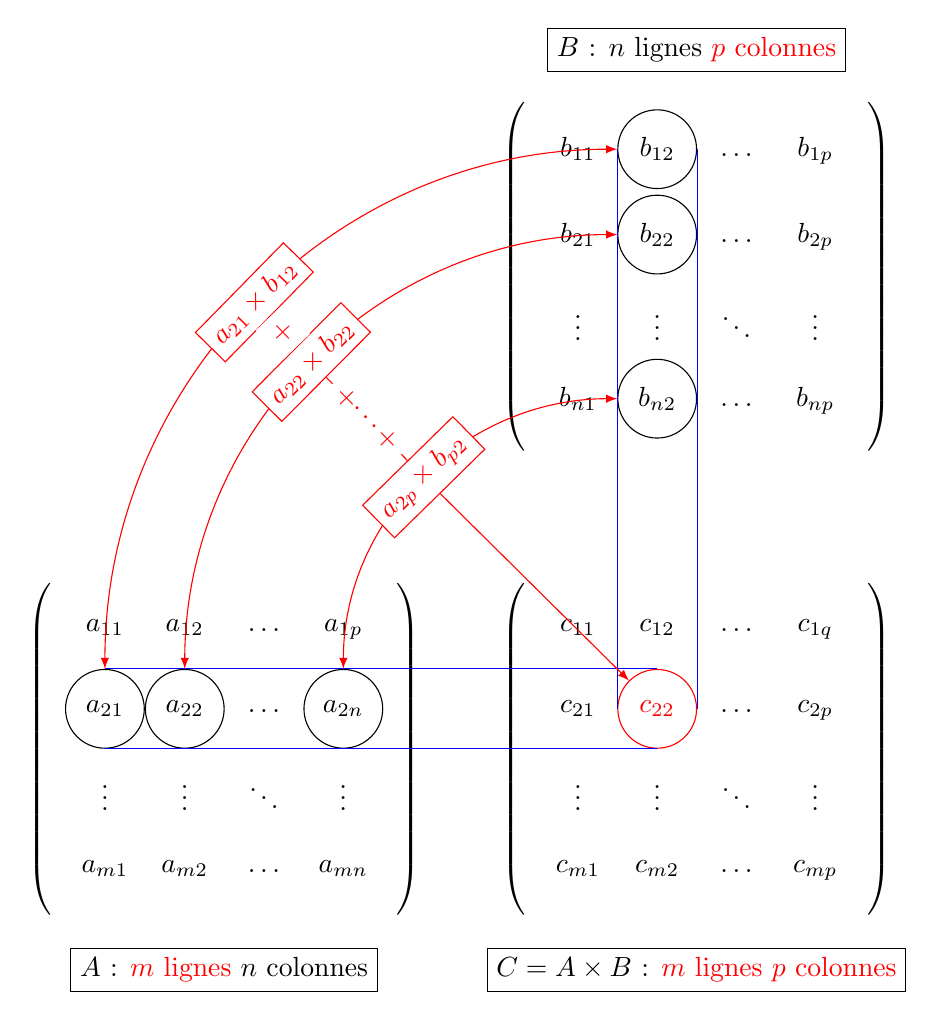
\begin{tikzpicture}[>=latex]
% les matrices
\matrix (A) [matrix of math nodes,%
             nodes = {node style ge},%
             left delimiter  = (,%
             right delimiter = )] at (0,0)
{%
  a_{11} & a_{12} & \ldots & a_{1p}  \\
  \node[node style sp](A-2-1) {a_{21}};%
         & \node[node style sp](A-2-2) {a_{22}};%
                  & \ldots%
                           & \node[node style sp](A-2-4) {a_{2n}}; \\
  \vdots & \vdots & \ddots & \vdots  \\
  a_{m1} & a_{m2} & \ldots & a_{mn}  \\
};
\node [draw,below=10pt] at (A.south) 
    { $A$ : \textcolor{red}{$m$ lignes} $n$ colonnes};

\matrix (B) [matrix of math nodes,%
             nodes = {node style ge},%
             left delimiter  = (,%
             right delimiter =)] at (6*\myunit,6*\myunit)
{%
  b_{11} & \node[node style sp](B-1-2) {b_{12}};%
                  & \ldots & b_{1p}  \\
  b_{21} & \node[node style sp](B-2-2) {b_{22}};%
                  & \ldots & b_{2p}  \\
  \vdots & \vdots & \ddots & \vdots  \\
  b_{n1} & \node[node style sp](B-4-2) {b_{n2}};%
                  & \ldots & b_{np}  \\
};
\node [draw,above=10pt] at (B.north) 
    { $B$ : $n$ lignes \textcolor{red}{$p$ colonnes}};
% matrice résultat
\matrix (C) [matrix of math nodes,%
             nodes = {node style ge},%
             left delimiter  = (,%
             right delimiter = )] at (6*\myunit,0)
{%
  c_{11} & c_{12} & \ldots & c_{1q} \\
  c_{21} & \node[node style sp,red](C-2-2) {c_{22}};%
                  & \ldots & c_{2p} \\
  \vdots & \vdots & \ddots & \vdots \\
  c_{m1} & c_{m2} & \ldots & c_{mp} \\
};
% les fleches
\draw[blue] (A-2-1.north) -- (C-2-2.north);
\draw[blue] (A-2-1.south) -- (C-2-2.south);
\draw[blue] (B-1-2.west)  -- (C-2-2.west);
\draw[blue] (B-1-2.east)  -- (C-2-2.east);
\draw[<->,red](A-2-1) to[in=180,out=90]
	node[arrow style mul] (x) {$a_{21}\times b_{12}$} (B-1-2);
\draw[<->,red](A-2-2) to[in=180,out=90]
	node[arrow style mul] (y) {$a_{22}\times b_{22}$} (B-2-2);
\draw[<->,red](A-2-4) to[in=180,out=90]
	node[arrow style mul] (z) {$a_{2p}\times b_{p2}$} (B-4-2);
\draw[red,->] (x) to node[arrow style plus] {$+$} (y)%
                  to node[arrow style plus] {$+\raisebox{.5ex}{\ldots}+$} (z)%
                  to (C-2-2.north west);


\node [draw,below=10pt] at (C.south) 
    {$ C=A\times B$ : \textcolor{red}{$m$ lignes}  \textcolor{red}{$p$ colonnes}};

\end{tikzpicture}
\end{center}


\begin{remarques}
\begin{itemize}
\item Le produit d'une matrice $A$ par une matrice $B$ n'existe qu'à condition que le nombre de colonnes de $A$ soit égale au nombre de lignes de $B$.
\item Si le produit d'une matrice $A$ par une matrice $B$ existe, en général, il n'est pas commutatif : en premier lieu, $BA$ n'existe pas toujours
(il n'existe que si $A$ et $B$ sont des matrices carrées) et, même si c'est le cas, généralement on n'a pas $AB=BA$.
\end{itemize}
\end{remarques}

\begin{methode}[Multiplier deux matrices]
Pour calculer la matrice $C$ égale à $AB$, on vérifie que le nombre de colonnes de $A$ est égal au nombre de lignes de $B$, puis on dispose
les matrices suivant le schéma
\begin{tabular}{c|c}
 & $B$ \\
 \hline
$A$ & $C$
\end{tabular} de sorte que  $c_{ij}$ soit à l'intersection du prolongement de la $i$-ème ligne de $A$ et de la $j$-ième colonne de $B$.


\begin{exercice}
 Soit
 $A=\begin{pmatrix}
1 &  3 & 5 & -2 \\
-2 & 0 & -3 & 2
\end{pmatrix}$ et $B=\begin{pmatrix}
2 & 1  & -3 \\
3 &  -1 & 0 \\
0 & -2 & 2 \\
2 & -3 & -4
\end{pmatrix}$. Calculer $AB$.

\begin{solution}

\begin{minipage}{0.5\linewidth}
$A$ est de taille $2\times4$ et $B$ de taille $4\times3$.\\
$A$ a autant de colonnes que $B$ a de lignes, donc $C=AB$ existe et sa taille est $2\times3$.\\
On dispose les matrices comme ci-contre.\\
On calcule alors, par exemple :\\
$c_{11}=\textcolor{B2}{\mathbf{1\times2+3\times3+5\times0-2\times2=7}}$.
\end{minipage}
\hfill
\begin{minipage}{0.45\linewidth}
\begin{tabular}{cc}
 & $\begin{pmatrix}
\textcolor{B2}{\mathbf{2}} & 1  & -3 \\
\textcolor{B2}{\mathbf{3}} &  -1 & 0 \\
\textcolor{B2}{\mathbf{0}} & -2 & 2 \\
\textcolor{B2}{\mathbf{2}} & -3 & -4
\end{pmatrix}$\\
$\begin{pmatrix}
\textcolor{B2}{\mathbf{1}} &  \textcolor{B2}{\mathbf{3}} & \textcolor{B2}{\mathbf{5}} & \textcolor{B2}{\mathbf{-2}} \\
-2 & 0 & -3 & 2
\end{pmatrix}$ & $\begin{pmatrix}
\textcolor{B2}{\mathbf{7}} & -6  & 15 \\
0 &  -2 & -8 \\
\end{pmatrix}$
\end{tabular}\\
\end{minipage}
\end{solution}
\end{exercice}
\end{methode}

\begin{remarque}
Il n'est pas nécessaire que l'une des matrices $A$ ou $B$ soit nulle pour que $AB\!=\!0$.
\end{remarque}

\begin{exemple}
Soit $A=\begin{pmatrix}1 & -1 \\ 0 & 0\end{pmatrix}$ et $B=\begin{pmatrix}1 & 2 & 3 \\ 1 & 2 & 3\end{pmatrix}$. Alors, $AB=\begin{pmatrix}0 & 0 & 0 \\ 0 & 0 & 0\end{pmatrix}$.
\end{exemple}

\begin{proprietes}
Soit $A$, $B$ et $C$ trois matrices compatibles avec les produits écrits ci-après et soit $k$ un réel.
\begin{itemize}
\item $(AB)C = A(BC) = ABC$ (associativité)
\item $A(B+C)=AB+AC$ et $(A+B)C=AC+BC$ (distributivité)
\item $(kA)B=A(kB)=k(AB)$
\item $AI=IA=A$ et $A0=0A=0$
\end{itemize}
\end{proprietes}

\subsection{Puissance d'une matrice carrée}

\begin{definition}
Soit $A$ une matrice carrée et $n$ un entier naturel.\\
La puissance $n$-ième de $A$ est la matrice notée $A^n$ égale :
\begin{itemize}
\item au produit de $n$ facteurs $A$ si $n\neq0$ ;
\item à la matrice identité $I$ de même ordre que celui de $A$ si $n=0$.
\end{itemize}
\end{definition}

\begin{exemple}
Soit $A=\begin{pmatrix}
 2 & 0 \\
0 & -3
\end{pmatrix}$.
Alors, $A^0=\begin{pmatrix}
 1 & 0 \\
0 & 1
\end{pmatrix}$ ; $A^2=\begin{pmatrix} 2 & 0 \\ 0 & -3 \end{pmatrix}\begin{pmatrix}  2 & 0 \\ 0 & -3 \end{pmatrix}=\begin{pmatrix}
 4 & 0 \\
 0 & 9
\end{pmatrix}$.\\
On peut démontrer par récurrence que, pout tout $n\in\mathbb{N}$,  $A^n=\begin{pmatrix}
 2^n & 0 \\
0 & (-3)^n
\end{pmatrix}$.\\
\end{exemple}

\begin{methode}[Effectuer un calcul matriciel avec la calculatrice]

 

\textbf{Exercice:}

 \renewcommand{\arraystretch}{0.9}
Soit
$A=\begin{pmatrix}
1 & -1 & 0 \\
0 & 1 & -1 \\
-1 & 0 & 1
\end{pmatrix}$ et $B=\begin{pmatrix}
3 & 2 & 1 \\
2 & 3 & 2 \\
1 & 2 & 3
\end{pmatrix}$. Calculer $A^2-2AB+B^2$.




\textbf{Correction}



\textcolor{H1}{\bfseries Avec une calculatrice TI % \raisebox{-1mm}{
\includegraphics[height=4mm]{TI_logo.eps}}
}
\begin{itemize}
\item Entrer dans le mode "Matrice"  puis le menu "EDIT".
\item Saisir la taille de la matrice $A$ puis ses coefficients. Pour les coefficients négatifs, utiliser la touche "(-)". Faire de même pour $B$.
\item Quitter le mode "Matrice" puis y entrer à nouveau et, dans le menu "NOMS", sélectionner la matrice 
\includegraphics[height=4mm]{TI_[A].eps}.
Compléter la formule et taper "Entrer".
 \begin{center}
   \fbox{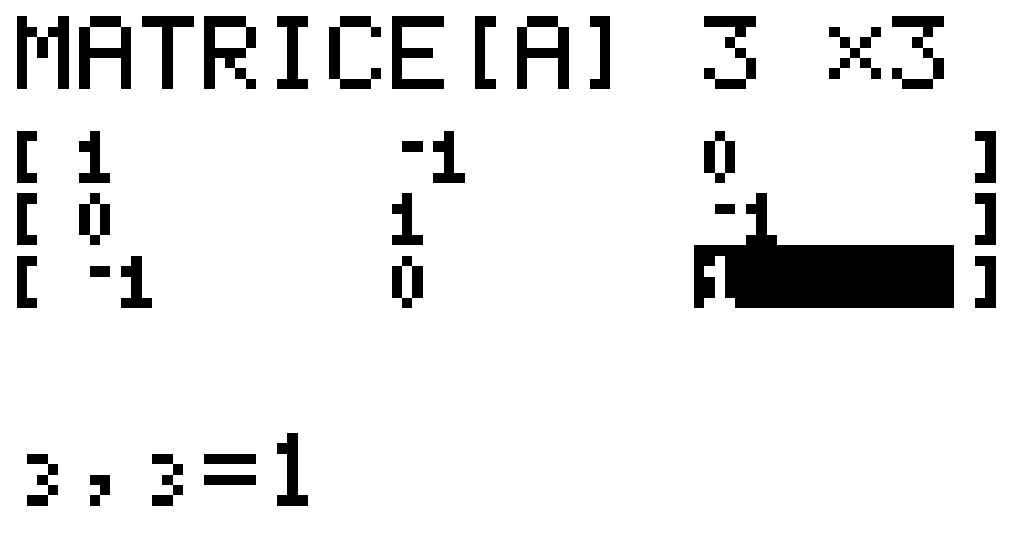
\includegraphics[height=2.cm]{TI_screenshot1.eps}} \hspace{.5cm} \fbox{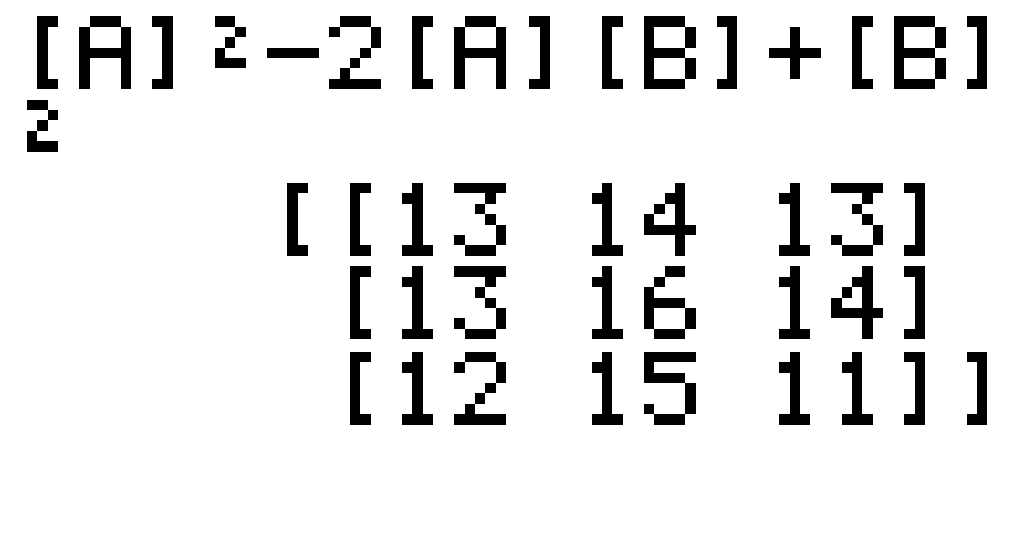
\includegraphics[height=2.cm]{TI_screenshot2.eps}}
   \end{center}
\end{itemize}

\textcolor{H1}{\bfseries Avec une calculatrice 
\includegraphics[height=2mm]{CASIO_logo.eps}}
\begin{itemize}
\item Entrer dans le menu "RUN-MAT" puis choisir 
\includegraphics[height=3mm]{CASIO_MAT.eps} (touche \touchecalc{F3}).
\item Saisir la taille de la matrice $A$ puis ses coefficients. Faire de même pour $B$.
\item Quitter 
\includegraphics[height=3mm]{CASIO_MAT.eps}, taper la formule en faisant précéder chaque nom de matrice par "Mat" (touches \touchecalc{SHIFT} puis \touchecalc{2}) : 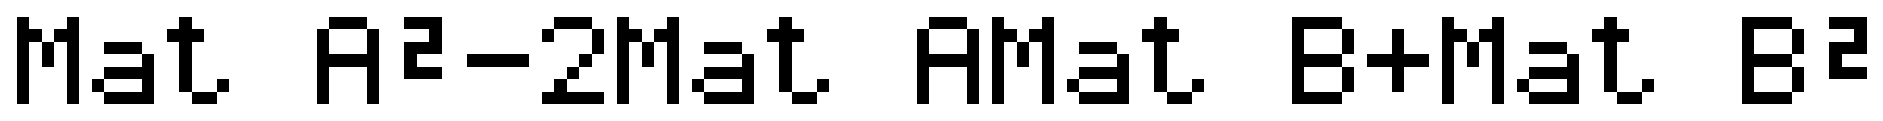
\includegraphics[height=3mm]{CASIO_screenshot2.eps}. Exécuter.
\begin{center}
   \fbox{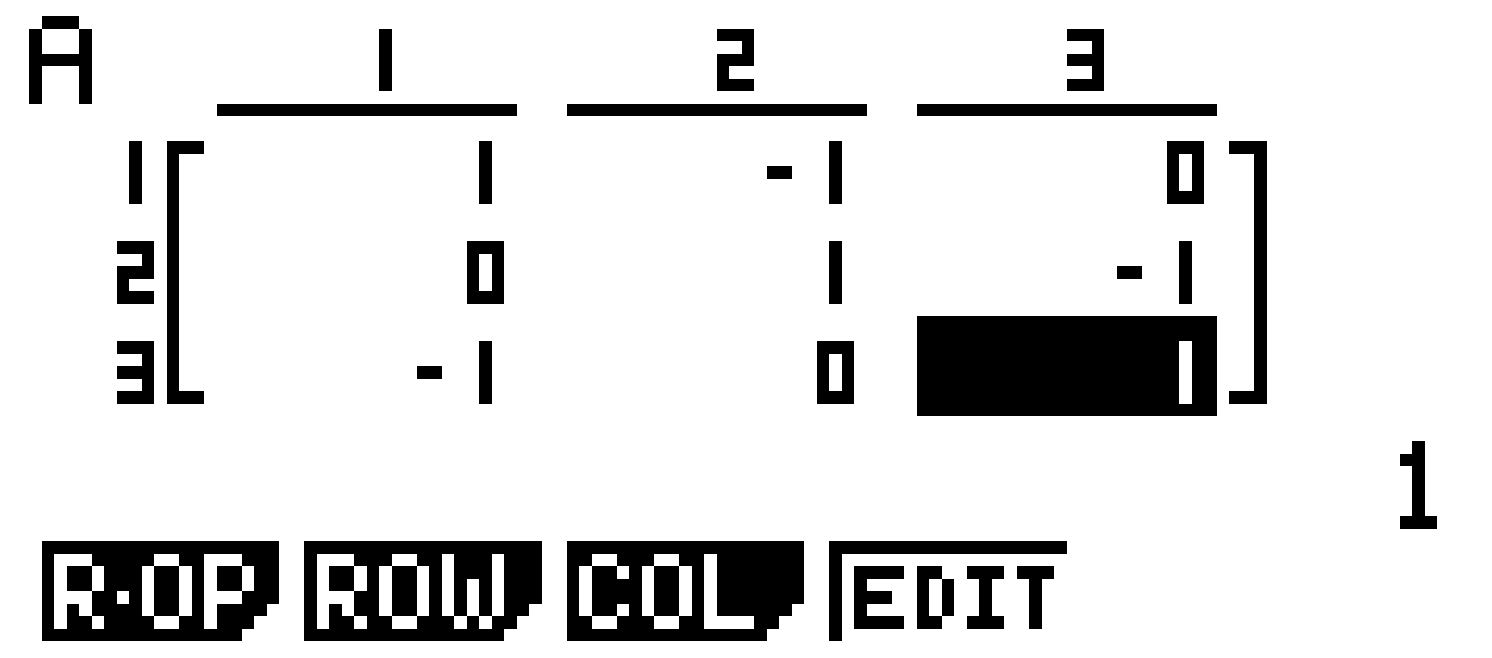
\includegraphics[height=2.cm]{CASIO_screenshot1.eps}}
    \hspace{.5cm} \fbox{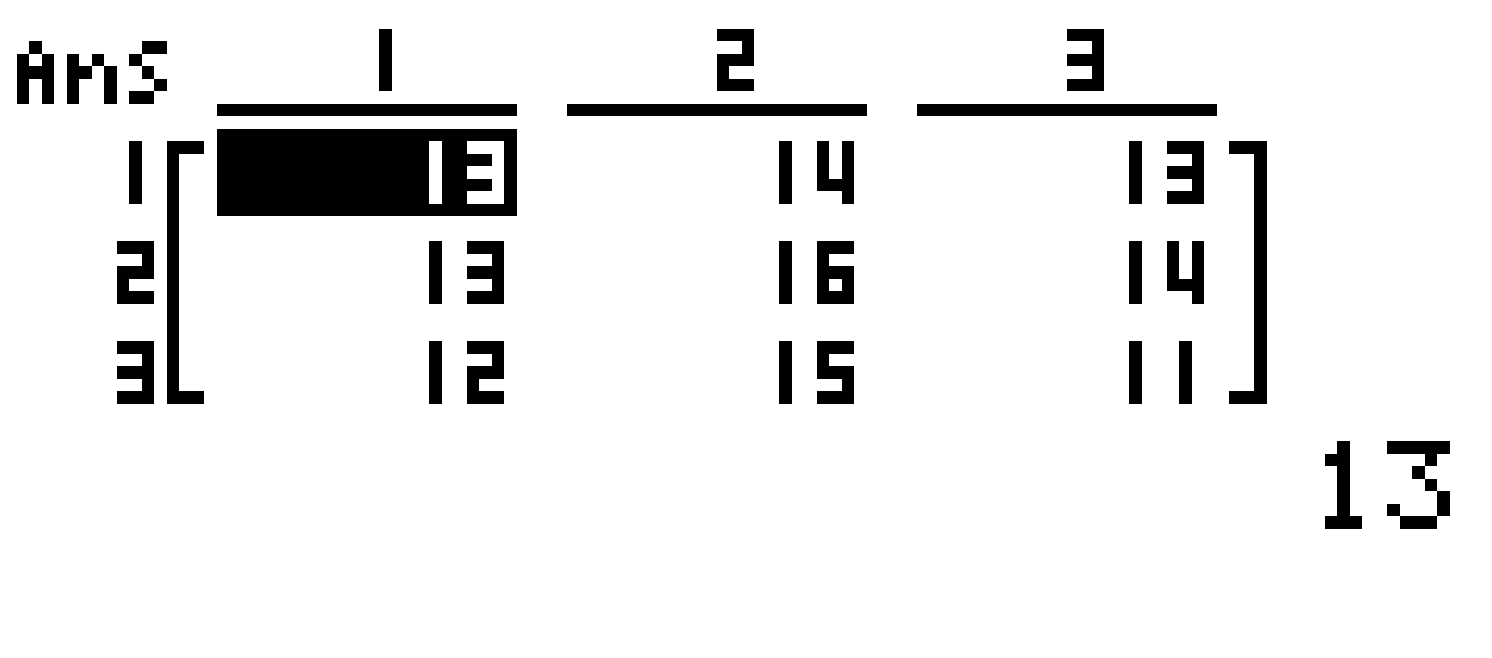
\includegraphics[height=2.cm]{CASIO_screenshot3.eps}}
   \end{center}
\end{itemize}

\end{methode}


\section{Matrices inversibles}

\subsection{Inverse d'une matrice carrée}

\begin{definition}[Inverse d'une matrice carrée]
Une matrice carrée $A$ d’ordre $n$ est \textbf{inversible} s’il existe une matrice carrée $B$ d’ordre $n$ telle que $AB=BA=I$.\\
La matrice $B$, notée $\boldsymbol{A^{-1}}$, est appelée la
\textbf{matrice inverse} de $A$.
\end{definition}

\begin{exemple}\setlength{\arraycolsep}{3.5pt}
Soit $A\hskip-.5mm=\hskip-.5mm\begin{pmatrix}
 3 & 5 \\
4 & 7
\end{pmatrix}$ et $B\hskip-.5mm=\hskip-.5mm\begin{pmatrix}
 7 & -5 \\
-4 & 3
\end{pmatrix}$. $AB\hskip-.5mm=\hskip-.5mmBA\hskip-.5mm=\hskip-.5mm\begin{pmatrix}
 1 & 0 \\
0 & 1
\end{pmatrix}$ donc $B$ est l'inverse de $A$.
\end{exemple}

\begin{propriete}
Si une matrice est inversible, alors son inverse est unique.
\end{propriete}

\begin{preuve}
Soit $A$ une matrice inversible ayant deux inverses  $B$ et $C$.\\
On a $B=BI=B(AC)=(BA)C=IC=C$. Ainsi, $B=C$. Donc, l'inverse de $A$ est unique.
\end{preuve}



\begin{propriete}
Si $AB=I$, alors $A$ est inversible et $B=A^{-1}$.
\end{propriete}

\begin{remarque}
Il suffit donc  seulement  de vérifier l'une des égalités $AB=I$ ou $BA=I$ pour montrer que $A$ et $B$ sont inverses l'une de l'autre.
\end{remarque}

\begin{exemple}
\renewcommand{\arraystretch}{0.9}
Soit $A=\begin{pmatrix}
1 & 1  & 0\\
-2 & -1 & 0 \\
3 & -2 & 1
\end{pmatrix}$ et
$B=\begin{pmatrix}
-1 & -1 & 0 \\
2 & 1 & 0 \\
7 & 5 & 1
\end{pmatrix}$. Alors, $AB=\begin{pmatrix}
 1 & 0 & 0\\
0 & 1 & 0 \\
0 & 0 & 1
\end{pmatrix}=I$.\\
Donc $A$ et $B$ sont inverses l'une de l'autre et on a les égalités $A^{-1}=B$ et $B^{-1}=A$.
\end{exemple}


\subsection{Inverse d'une matrice carrée d'ordre 2}

\begin{definition}[Déterminant d'une matrice carrée d'ordre 2]
Le \textbf{déterminant} de la matrice $M=\begin{pmatrix}
 a & b \\
c & d
\end{pmatrix}$ est le réel noté $\det(M)$ ou $\begin{vmatrix}
 a & b \\
c & d
\end{vmatrix}$ égal à $ad-bc$.
\end{definition}


\begin{theoreme}[Inverse d'une matrice carrée d'ordre 2]
On prend $M \neq 0$.
\begin{itemize}
\item La matrice $M=\begin{pmatrix}
 a & b \\
c & d
\end{pmatrix}$  est inversible si, et seulement si, $ad-bc\neq0$.\\
\item Si $A$ est inversible, alors $A^{-1}=\dfrac{1}{ad-bc}\begin{pmatrix}
 d & -b \\
-c & a
\end{pmatrix}=\dfrac{1}{\text{det}(A)}\begin{pmatrix}
 d & -b \\
-c & a
\end{pmatrix}$.
\end{itemize}
\end{theoreme}

\begin{preuve}\setlength{\arraycolsep}{3.5pt}
Soit $N=\begin{pmatrix}
 d & -b \\
-c & a
\end{pmatrix}$. Alors,
$MN=\begin{pmatrix}
 a & b \\
c & d
\end{pmatrix}
\begin{pmatrix}
 d & -b \\
-c & a
\end{pmatrix}=
\begin{pmatrix}
 ad-bc & 0 \\
0 & ad-bc
\end{pmatrix}
$.
\begin{itemize}
\item Si $ad-bc\neq0$, alors $\dfrac{1}{ad-bc}MN=I\Leftrightarrow M\left(\dfrac{1}{ad-bc}N\right)=I$.\\
Donc $M$ est inversible et son inverse est $\dfrac{1}{ad-bc}N=\dfrac{1}{ad-bc}
\begin{pmatrix}
 d & -b \\
-c & a
\end{pmatrix}$.
\item Si $ad-bc=0$, alors $MN=0$. Supposons alors que $M$ soit inversible, d'inverse $P$.\\
    Alors, on aurait $PMN=IN=N$ et  $PMN=P0=0$ et donc $N=0$, ce qui est absurde car $M \neq 0$.
\item On a donc montré que si $ad-bc \neq 0$ alors $M$ est inversible, et si $ad-bd=0$ alors $M$ n'est pas inversible. On obtient donc l'équivalence demandée.
\end{itemize}
\end{preuve}

\begin{remarque}
Un peu logique: si $A$  et $B$ sont deux propositions, alors $(A \Rightarrow B) \iff (\text{non}(B) \Rightarrow \text{non}(A))$\newline
En revenant à la démonstration prédente: notons $A$ la proposition "$ad-bc \neq 0$" et $B$ la proposition "$M$ est inversible"\newline
On montre dans un premier temps que $A \Rightarrow B$\newline
On montre ensuite que $\text{non}(A) \Rightarrow \text{non}(B)$, ce qui nous donne bien $B \Rightarrow A$.
\end{remarque}

\begin{remarques}
\begin{itemize}
\item Toute matrice carrée admet un déterminant et un seul, mais pour un ordre strictement supérieur à 2,
il n'existe pas de formule simple pour le calculer et on utilisera une calculatrice ou un logiciel de calcul formel.
\item Le déterminant non nul est un critère d'inversibilité d'une matrice carrée de tout ordre.
\end{itemize}
\end{remarques}

\begin{exemple}
$A=\begin{pmatrix}
 3 & 8 \\
2 & 6\end{pmatrix}$. Alors, $\det(A)=\begin{vmatrix}
 3 & 8 \\
2 & 6
\end{vmatrix}=3\times6-2\times8=18-16=2\neq0$.\\
Ainsi, $A$ est inversible et $A^{-1}=\dfrac{1}{2}
\begin{pmatrix}
 6 & -8 \\
-2 & 3\end{pmatrix}=\begin{pmatrix}
 3 & -4 \\
-1 & 1,5\end{pmatrix}$.
\end{exemple}


\section{Résolution d'un système linéaire}

\begin{propriete}[Écriture matricielle d'un système]
Le système linéaire
$\left\{\begin{array}{ccc}
ax+by & = & c\\
a'x+b'y & = & c'
\end{array}\right.$
 a pour écriture matricielle
$\begin{pmatrix}
 a & b \\
 a' & b'\end{pmatrix}\begin{pmatrix}
 x  \\
y \end{pmatrix}=\begin{pmatrix}
 c  \\
c' \end{pmatrix}$.
\end{propriete}

\begin{preuve}
$\begin{pmatrix}
 a & b \\
 a' & b'\end{pmatrix}\begin{pmatrix}
 x  \\
y \end{pmatrix}=\begin{pmatrix}
 c  \\
c' \end{pmatrix}
\Leftrightarrow
\begin{pmatrix}
 ax+by \\
 a'x+b'y\end{pmatrix}
=\begin{pmatrix}
 c  \\
c' \end{pmatrix}
\Leftrightarrow
\left\{\begin{array}{ccc}
ax+by & = & c\\
a'x+b'y & = & c'
\end{array}\right.$.
\end{preuve}

\begin{remarque}
Cette propriété se généralise à un système  de dimension quelconque.
\end{remarque}




\begin{exemple}
$\begin{pmatrix}
 2 & -3 & 1 \\
 3 & -2 & -1 \end{pmatrix}\begin{pmatrix}
 x  \\
y \\
z \end{pmatrix}=\begin{pmatrix}
 7  \\
-5 \end{pmatrix}$ correspond au système
$\left\{\begin{array}{ccc}
2x-3y+z & = & 7\\
3x-2y-z & = & -5
\end{array}\right.$.
\end{exemple}


\begin{propriete}
Soit $A$ une matrice carrée inversible d'ordre $n$ et $B$ une matrice colonne de taille $n$.\\
Alors, le système linéaire d'écriture matricielle $AX=B$ admet une unique solution :\\
le $n$-uplet  correspondant à la matrice colonne $A^{-1}B$.
\end{propriete}

\begin{preuve}
Soit un système linéaire d'écriture matricielle $AX=B$ où $A$ est inversible.\\
Alors, on a  :
$AX=B \Leftrightarrow A^{-1}AX = A^{-1}B \Leftrightarrow
IX=A^{-1}B \Leftrightarrow X=A^{-1}B$.
\end{preuve}


\begin{methode}[Résoudre un système de deux équations à deux inconnues ]
 

\textbf{Exercice:}

 \label{TMS1_M_resolution_systeme0}
Résoudre le système linéaire  $\left\{\begin{array}{lcc}
2x+5y & = & 8 \\
3x-4y & = & 15
\end{array}\right. $.


\textbf{Correction}


On résout l'équation $AX=B$ où
$A=\begin{pmatrix}
   2 & 5 \\
   3 & -4
 \end{pmatrix}$, $X=\begin{pmatrix}
   x \\
   y
 \end{pmatrix}$ et   $B=\begin{pmatrix}
   8 \\
   15
\end{pmatrix}$.\\
On calcule $\det(A)=-4\times2-3\times5=-23$. Comme $\det(A)\neq0$, alors $A$ est inversible.\\
Donc, l'équation $AX=B$ a pour unique solution $X=A^{-1}B$.\\
On calcule $X=\dfrac{-1}{23}\begin{pmatrix} -4 & -5 \\
   -3 & 2
 \end{pmatrix}\begin{pmatrix}
   8 \\
   15
\end{pmatrix}=\dfrac{-1}{23}\begin{pmatrix} -4\times8-5\times15 \\ -3\times8+2\times15\end{pmatrix}=\begin{pmatrix}107/23 \\ -6/23 \end{pmatrix}$.\\
Le système admet donc pour unique solution le couple $\left(\dfrac{107}{23}~;~\dfrac{-6}{23}\right)$.
\end{methode}

\begin{remarque}
Un système linéaire d'écriture matricielle $AX=B$ où $A$ n'est pas inversible a soit une infinité de solutions, soit aucune.
\end{remarque}




\begin{exemple}
Le système $\left\{\begin{array}{lcc}
3x+6y & = & a \\
4x+8y & = & b
\end{array}\right.$ s'écrit matriciellement $AX=B$ où $A=\begin{pmatrix}
   3 & 6 \\
   4 & 8
 \end{pmatrix}$.\\
 Or, $\det(A)=0$ donc $A$ n'est pas inversible.\\
 Dans le système, multiplions l'équation du haut par 4 et celle du bas par 3. On obtient :\\
 $\left\{\begin{array}{lcc}
12x+24y & = & 4a \\
12x+24y & = & 3b
\end{array}\right.$ ce qui entraîne que $4a=3b$ toujours vrai, ou jamais.
\end{exemple}


\end{document}